\documentclass[aspectratio=169,14pt,usenames,dvipsnames]{beamer}
\usetheme{TalentSprint}
\usepackage[utf8]{inputenc}
\usepackage{graphics}
\usepackage{ragged2e}
\usepackage{amsfonts}
\usepackage{xcolor}
\usepackage{mathtools}
\usepackage{tcolorbox}
\usepackage{setspace}
\usepackage{lmodern}
\usepackage{hyperref}
\definecolor{swe}{rgb}{0.19, 0.73, 0.56}
\definecolor{lgreen}{RGB}{190,200,198}
\title[Features and Dimensions]{Features and Dimensions}

\begin{document}

{\1
\begin{frame} \vspace{35pt}
	\maketitle
\end{frame}
}

\begin{frame}{Data volume}
\begin{itemize}
  \item For machine learning, more data is always better \break
\setbeamertemplate{itemize, items}[circle]
\begin{itemize}
\itemsep1em 
\item Defined data distribution 
\item Outliers easy to identify 
\item More accurate models
\end{itemize}
\end{itemize}
\end{frame}

\begin{frame}{Data features}
\begin{itemize}
\item What about more features (dimensions) of data? \break
\setbeamertemplate{itemize, items}[circle]
\begin{itemize}
\itemsep1em 
\item Not necessarily desirable
\item Most of the variability in a model can be explained by a few features
\end{itemize}
\end{itemize}
\end{frame}

\begin{frame}{Curse of dimensionality}
\begin{itemize}
\item With each additional dimension, sparsity increases and the number of samples needed to achieve high accuracy grows exponentially\\
\end{itemize}
\centering
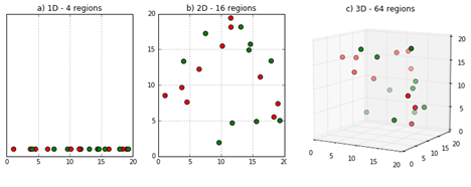
\includegraphics[width=12.5cm , height=3.5cm]{Images/AIML_FD_IMG1.png}
\end{frame}

\begin{frame}{High dimensional data issues}
\begin{itemize}
\item Data is highly sparse
\item Data cannot be visualized well
\item More training time required
\item High risk of overfitting
\item Lower prediction accuracy
\end{itemize}
\end{frame}

\begin{frame}{Reducing Dimensions}
\begin{columns}
\column{0.5\textwidth}
\begin{itemize}
\color{Red}
\item Feature Selection
\setbeamertemplate{itemize items}[-]
\begin{itemize}
\item The "best features" are selected or the irrelevant features are discarded
\end{itemize}
\end{itemize}
\begin{itemize}
\color{Red}
\item Feature Extraction
\setbeamertemplate{itemize, items}[-]
\begin{itemize}
\item The existent variables are combined to  form new features
\end{itemize}
\end{itemize}
\column {0.5\textwidth}
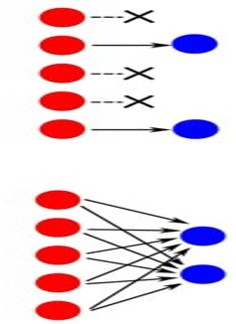
\includegraphics[width=0.4\textwidth, height=0.7\textheight]{Images/AIML_FD_IMG2.jpg}
\end{columns}
\end{frame}

\begin{frame}{}
\centering
\color{orange}
\large Feature Selection
\end{frame}

\begin{frame}{Usefulness of features}
\begin{itemize}
\item How do you know which features are useful and which are not?\\
\end{itemize}
\centering
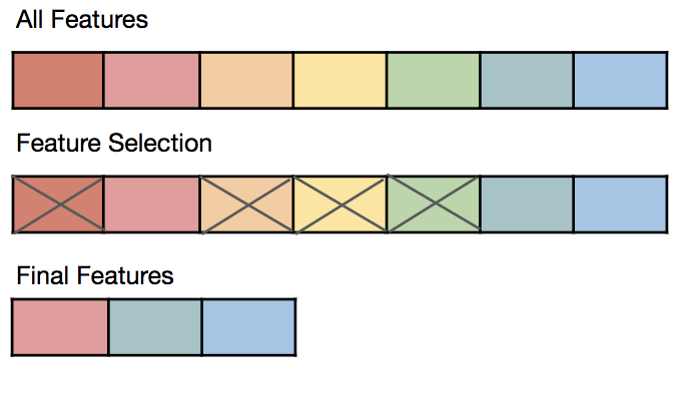
\includegraphics[width=8cm , height=3.5cm]{Images/AIML_FD_IMG3.png}

\end{frame}

\begin{frame}{Techniques for feature selection}
\begin{itemize}
\item "All But X" - Features are removed one at a time and the model accuracy is measured. The features that did not affect the model performance are removed from the final set\\
\end{itemize}
\centering
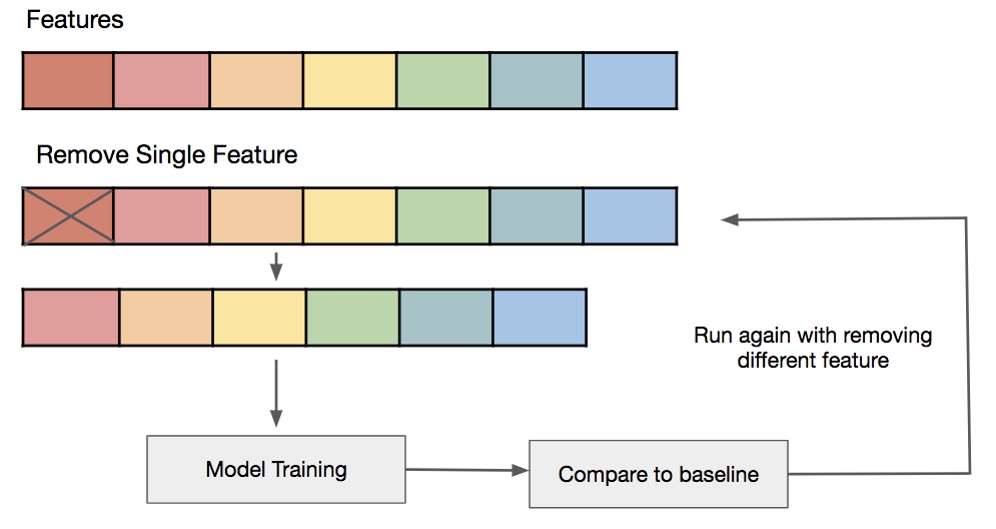
\includegraphics[width=10cm , height=4cm]{Images/AIML_FD_IMG4.png}
\end{frame}

\begin{frame}{Techniques for feature selection}
\begin{itemize}
\item Filter method – Features that show a statistically significant correlation with the target (dependent) variable are selected\\
\end{itemize}
\centering
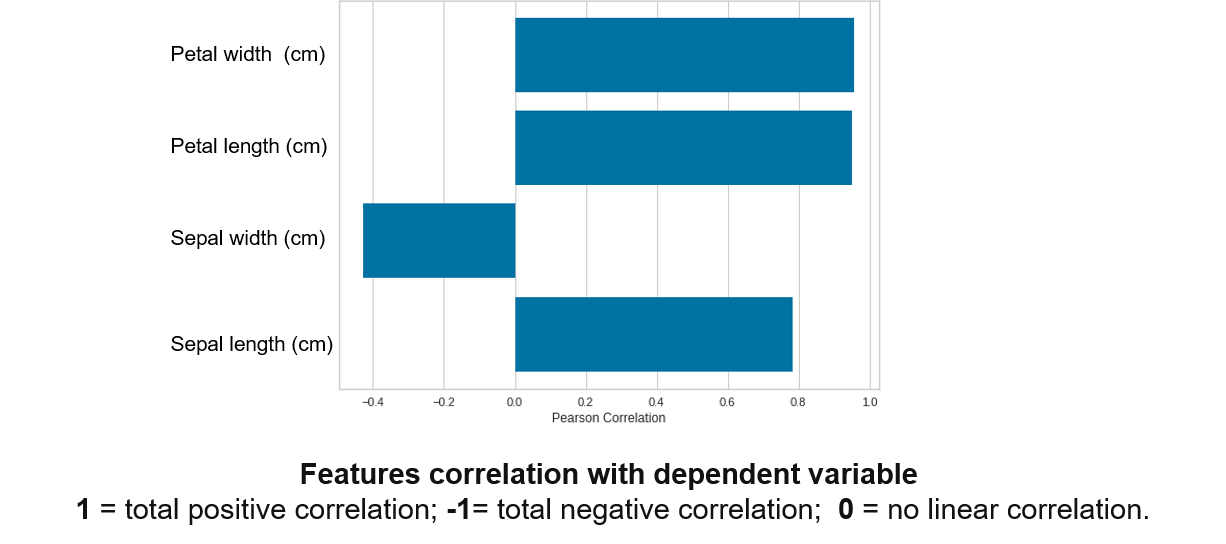
\includegraphics[width=10.5cm , height=4cm]{Images/AIML_FD_IMG5.png}

\end{frame}

\begin{frame}{Deeper Look}
\centering
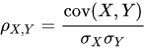
\includegraphics[width=6.5cm , height=2.5cm]{Images/AIML_FD_IMG6.png}
\end{frame}

\begin{frame}{Techniques for feature Selection: Filter Method}
\begin{itemize}
\item High Correlation filter – Firstly, the highly correlated input variables are identified\\
\end{itemize}
\centering
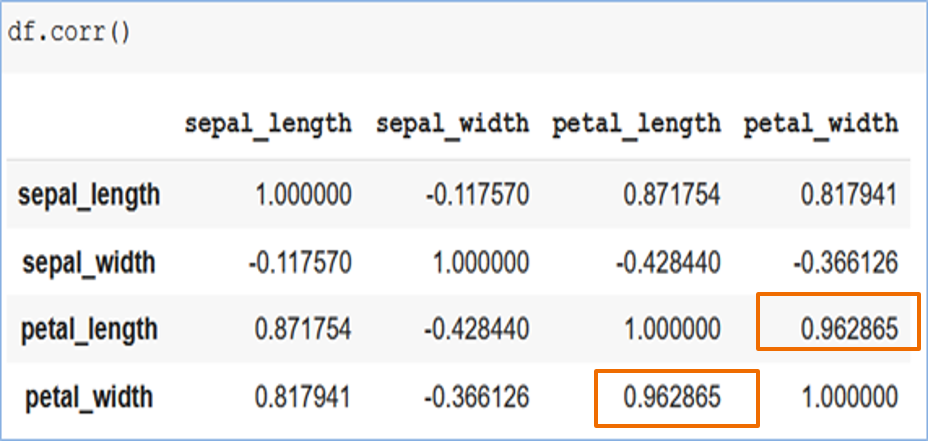
\includegraphics[width=10cm , height=4cm]{Images/AIML_FD_IMG7.png}
\end{frame}


\begin{frame}{Techniques for feature selection: Filter method}
\begin{itemize}

\item High Correlation filter – The highly correlated input variables that have a weaker correlation with the target variable are discarded\\
\end{itemize}
\centering
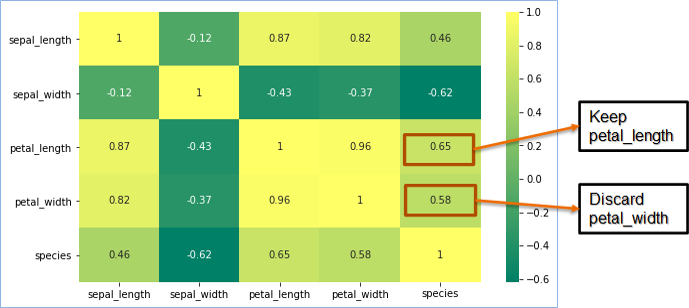
\includegraphics[width=10cm , height=4cm]{Images/AIML_FD_IMG8.png}
\end{frame}

\begin{frame}{Techniques for feature selection}
\begin{itemize}
\item Wrapper method: A subset of features is used to train a model and select or remove the features based on inferences from each model's performance.\\
\item Usually computationally very expensive
\end{itemize}
\centering
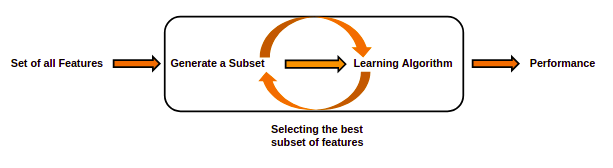
\includegraphics[width=14cm , height=3.5cm]{Images/AIML_FD_IMG9.png}
\end{frame}

\begin{frame}{Techniques for feature selection: Wrapper method}
\begin{itemize}
\item Recursive feature elimination
\setbeamertemplate{itemize, items}[-]
\begin{itemize}
\item The best or the worst performing feature at each iteration is saved
\item The next model is constructed with the remaining features until all the features are exhausted
\item The features are ranked based on the order of their elimination
\end{itemize}
\end{itemize}
\end{frame}

\begin{frame}{Feature Selection: Summary}
\begin{itemize}
\item Important part of part of feature engineering\\
- the number of input variables is reduced\\
- the computational cost of modeling is reduced\\
- the performance of the model improves in some cases\\

\item Filter methods select input variables that have a strong correlation with the target variable
\item Wrapper methods provide the best subset of features
\item Feature selection is less critical in these days of Deep Learning
\end{itemize}
\end{frame}

\begin{frame}{}
\centering
\color{orange}
\large Feature Extraction
\end{frame}

\begin{frame}{Reducing Dimensions}
\begin{columns}
\column{0.5\textwidth}
\begin{itemize}
\color{Red}
\item Feature Selection
\setbeamertemplate{itemize, items}[-]
\begin{itemize}
\item The "best features" are selected or the irrelevant features are discarded
\end{itemize}
\end{itemize}
\begin{itemize}
\color{Red}
\item Feature Extraction
\begin{itemize}
\item The existent variables are combined to  form new features
\end{itemize}
\end{itemize}
\column {0.5\textwidth}
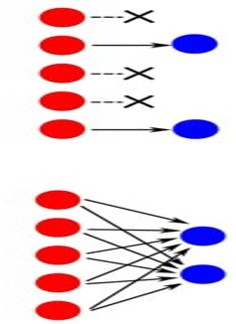
\includegraphics[width=0.4\textwidth, height=0.7\textheight]{Images/AIML_FD_IMG2.jpg}
\end{columns}
\end{frame}

\begin{frame}{Feature Extraction}
\begin{itemize}
\item Builds derived features from the initial set of measured data \break
\item Helps to
\begin{itemize}
\item visualize data in 2D/3D
\item remove some 'useless' or 'less useful' features
\item make computations efficient
\begin{itemize}
\item Note: original data could be 1000s of dimensions
\end{itemize}
\end{itemize}
\end{itemize}
\end{frame}

\begin{frame}{Some angles are better than others}
\centering
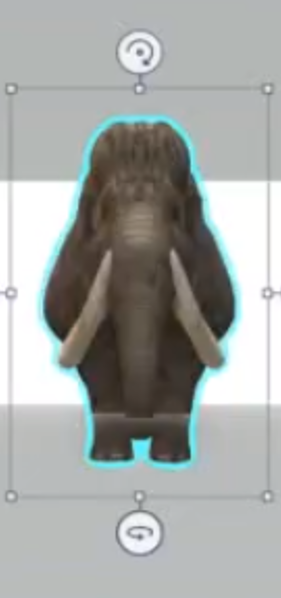
\includegraphics[width=3.5cm , height=5.5cm]{Images/AIML_FD_IMG10.png} 

\tiny
\href{https://cdn.exec.talentsprint.com/content/Mammoth 3D_without audio_cropped.mp4}{Wooly Mammoth}
\end{frame}

\begin{frame}{What is this object?}
\centering
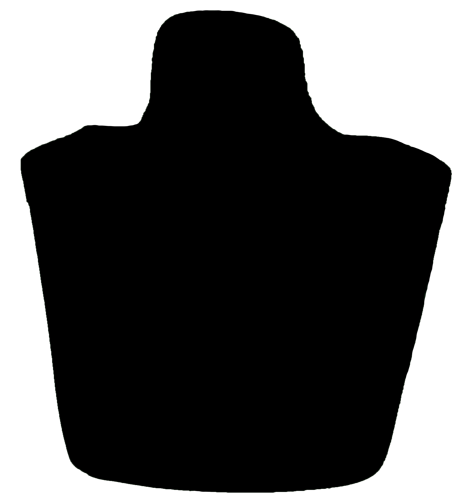
\includegraphics[width=4.5cm , height=3.5cm]{Images/IMG11.png}
\end{frame}


\begin{frame}[t]{Some angles are better than others}
	\begin{itemize}
		\item Which is the best angle?  \break \break \break \break \break
	\end{itemize}
	\begin{tikzpicture} 
		\only<1-> 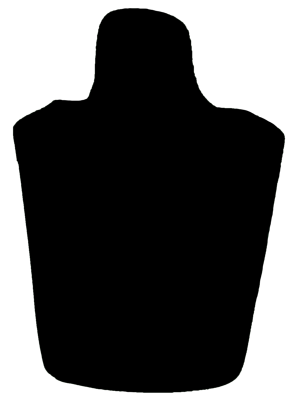
\includegraphics[width=3.5cm, height=2.9cm]{Images/IMG12.png}
		\only<2-> 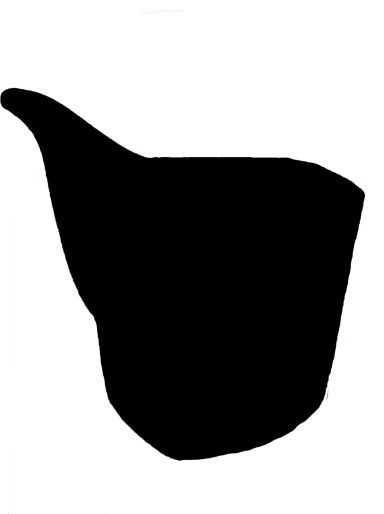
\includegraphics[width=3.5cm, height=2.9cm]{Images/IMG13.png}
                \only<3-> 
\includegraphics[width=3.5cm, height=2.9cm]{Images/IMG14.png}
                \only<4-> 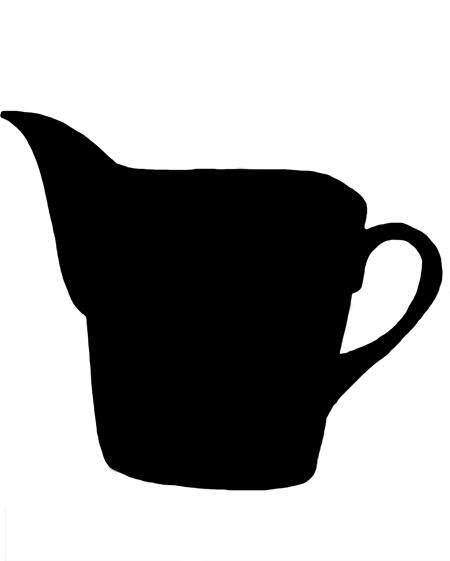
\includegraphics[width=3.5cm, height=2.9cm]{Images/IMG15.png}
	\end{tikzpicture}
\end{frame}
		
\begin{frame}{Feature representation}
\begin{itemize}
\item How would you obtain the best angle or representation?
\end{itemize}
\centering
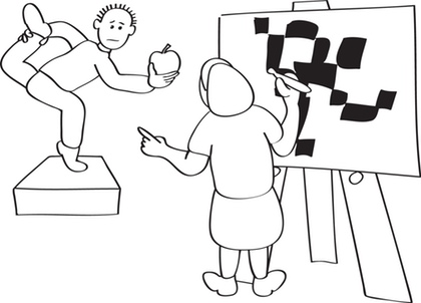
\includegraphics[width=4.8cm , height=3.8cm]{Images/AIML_FD_IMG16.png}\\

\tiny classic.csunplugged.org
\end{frame}


\begin{frame}{A motivating example}
\begin{itemize}
\item Plot height vs weight in children
\item How will it look?
\item What can we change it to?
\end{itemize}
\end{frame}

\begin{frame}{Summary}
\begin{itemize}
\item Feature Extraction
\setbeamertemplate{itemize, items}[-]
\begin{itemize}
\item Selects the direction of projection of data points from a higher dimension to a lower dimension, such that maximum variance is preserved
\item Thus derives new features from a combination of original features and reduces data dimensions
\end{itemize}
\end{itemize}
\end{frame}

{\1
\begin{frame}
	\title{Mathematically speaking!}
	\subtitle{Matrices are the key!!}
\titlepage
\end{frame}
}

\begin{frame}{Selecting Features as Matrix Multiplication}

	\hspace{3cm}	\only<1->{$X = \begin{bmatrix} x_1 \\ x_2 \\ x_3 \\ x_4 \end{bmatrix} $ \hspace{2cm}} \only<6->{\alert{Z = UX} } 
	
	\vspace{-0.7cm}
				
	\begin{itemize}
		\only<2>{\vspace{1cm}}
		\item<2-> {\small{Select first and third feature}}  \only<3->{\small{$
	 \begin{bmatrix}
	    z_1 \\
	    z_2 
	 \end{bmatrix}=\begin{bmatrix}
                     x_1 \\
                     x_3 
                    \end{bmatrix} = \begin{bmatrix} 
                                     1&0&0&0 \\ 
                                     0&0&1&0  \end{bmatrix} \begin{bmatrix}
                                     x_1 \\
                                     x_2 \\
                                     x_3 \\
	  x_4 \end{bmatrix} $}}
	\end{itemize}

\begin{itemize}
		\vspace{-0.18cm}	
	\item<4-> {\small{Select first and fourth feature}}   \only<5->{\small{ $ 
 \begin{bmatrix}
      z_1 \\
      z_2
      \end{bmatrix}= \begin{bmatrix} 
                      x_1 \\
                      x_4 
                      \end{bmatrix} = \begin{bmatrix} 
                                       1&0&0&0 \\
                                       0&0&0&1  \end{bmatrix} \begin{bmatrix} 
                                        x_1 \\
                                        x_2 \\
                                        x_3 \\
 x_4 \end{bmatrix}$}}  
\end{itemize}
\end{frame}


{ \1
\begin{frame}
	\title{Thanks!!}
	\subtitle{Questions?}
	\maketitle
\end{frame}
}

\end{document}
